\documentclass[twocolumn,a4paper,11pt]{scrartcl}

% Language and font encoding
\usepackage[spanish,es-noshorthands]{babel}
\usepackage[utf8]{inputenc}
\usepackage[T1]{fontenc}

% Other necessary packages
\usepackage{graphicx}
\usepackage{amsmath}
\usepackage{cite}

% Title information
\title{Óptica Geométrica}
\author{Nombre del Autor}
\date{}

\begin{document}

\maketitle

\begin{abstract}
Este trabajo presenta un estudio experimental sobre óptica geométrica, centrado en la verificación de la ecuación de lentes delgadas y el análisis de la magnificación de imágenes. Utilizando un montaje que incluía una fuente de luz, un objeto triangular, una lente delgada y una pantalla, se realizaron mediciones sistemáticas de las distancias objeto-lente e imagen-lente, así como de las alturas del objeto y su imagen. Los resultados obtenidos demuestran una estrecha correlación entre los valores experimentales y las predicciones teóricas, con una discrepancia promedio en la magnificación del X.X. La distancia focal calculada (F ± ΔF cm) coincidió con el valor nominal de la lente dentro del margen de error experimental. Se observó consistentemente la formación de imágenes invertidas cuando $s_o > f$, en línea con la teoría. Este estudio no solo valida los principios fundamentales de la óptica geométrica en condiciones de laboratorio, sino que también ilustra la importancia de considerar las incertidumbres experimentales en la interpretación de datos físicos.
\end{abstract}

\section{Objetivos}

Comprobar experimentalmente la validez de la ecuación de lentes delgadas, contrastando resultados de laboratorio con predicciones teóricas. Esto nos permitirá verificar la aplicabilidad de los modelos matemáticos en situaciones reales.

Determinar con precisión la distancia focal de una lente delgada mediante mediciones experimentales y cálculos basados en la ecuación de lentes, profundizando así en las propiedades ópticas de estos sistemas.

Analizar la magnificación de la imagen producida por una lente, comparando mediciones experimentales con valores teóricos para evaluar la precisión de nuestras predicciones.


\section{Marco teórico}
La óptica geométrica se basa en el principio de que la luz viaja en línea recta en medios homogéneos. Uno de los elementos fundamentales en este campo es la lente delgada, cuyo comportamiento se describe mediante la ecuación de lentes delgadas. Esta ecuación, como señala Serway et al. \cite{serway}, relaciona la distancia focal de la lente con las distancias del objeto y la imagen.

La ecuación de lentes delgadas se expresa como:

\begin{equation}
\frac{1}{f} = \frac{1}{s_o} + \frac{1}{s_i}
\end{equation}

Donde $f$ es la distancia focal de la lente, $s_o$ es la distancia del objeto a la lente, y $s_i$ es la distancia de la imagen a la lente. Esta ecuación es válida tanto para lentes convergentes como divergentes, y permite predecir la posición y características de la imagen formada por una lente delgada.

Además de la posición de la imagen, es importante considerar su tamaño en relación con el objeto. Esto se cuantifica mediante la magnificación $M$, definida como la relación entre el tamaño de la imagen y el tamaño del objeto:

\begin{equation}
M = -\frac{s_i}{s_o}
\end{equation}

El signo negativo en esta ecuación indica la orientación de la imagen con respecto al objeto. Una magnificación positiva implica una imagen derecha, mientras que una negativa indica una imagen invertida.

Estas ecuaciones fundamentales permiten analizar y predecir el comportamiento de sistemas ópticos simples, sentando las bases para el estudio de sistemas más complejos en óptica geométrica.

\section{Diseño experimental}
Para verificar experimentalmente la ecuación de lentes delgadas y analizar la magnificación, se empleó un conjunto de instrumentos especializados. El equipo utilizado incluyó:

\begin{itemize}
    \item Transformador 0 a 25 V 6A AC/DC (LH 522 20)
    \item Lámpara 6V 30W (LH 450 60)
    \item Porta objetos
    \item Objetos de varias figuras (se utilizó un triángulo)
    \item Lente de distancia focal conocida
    \item Pantalla traslúcida
    \item Jinetillos
    \item Riel Óptico
\end{itemize}

La configuración experimental, ilustrada en la Figura 1, constaba de cuatro elementos principales: una fuente de luz blanca, un objeto triangular, una lente delgada y una pantalla donde se proyectaba la imagen del triángulo. Esta disposición permitía una manipulación precisa de las distancias entre los componentes y una observación clara de la imagen formada.

\begin{figure}[h]
    \centering
    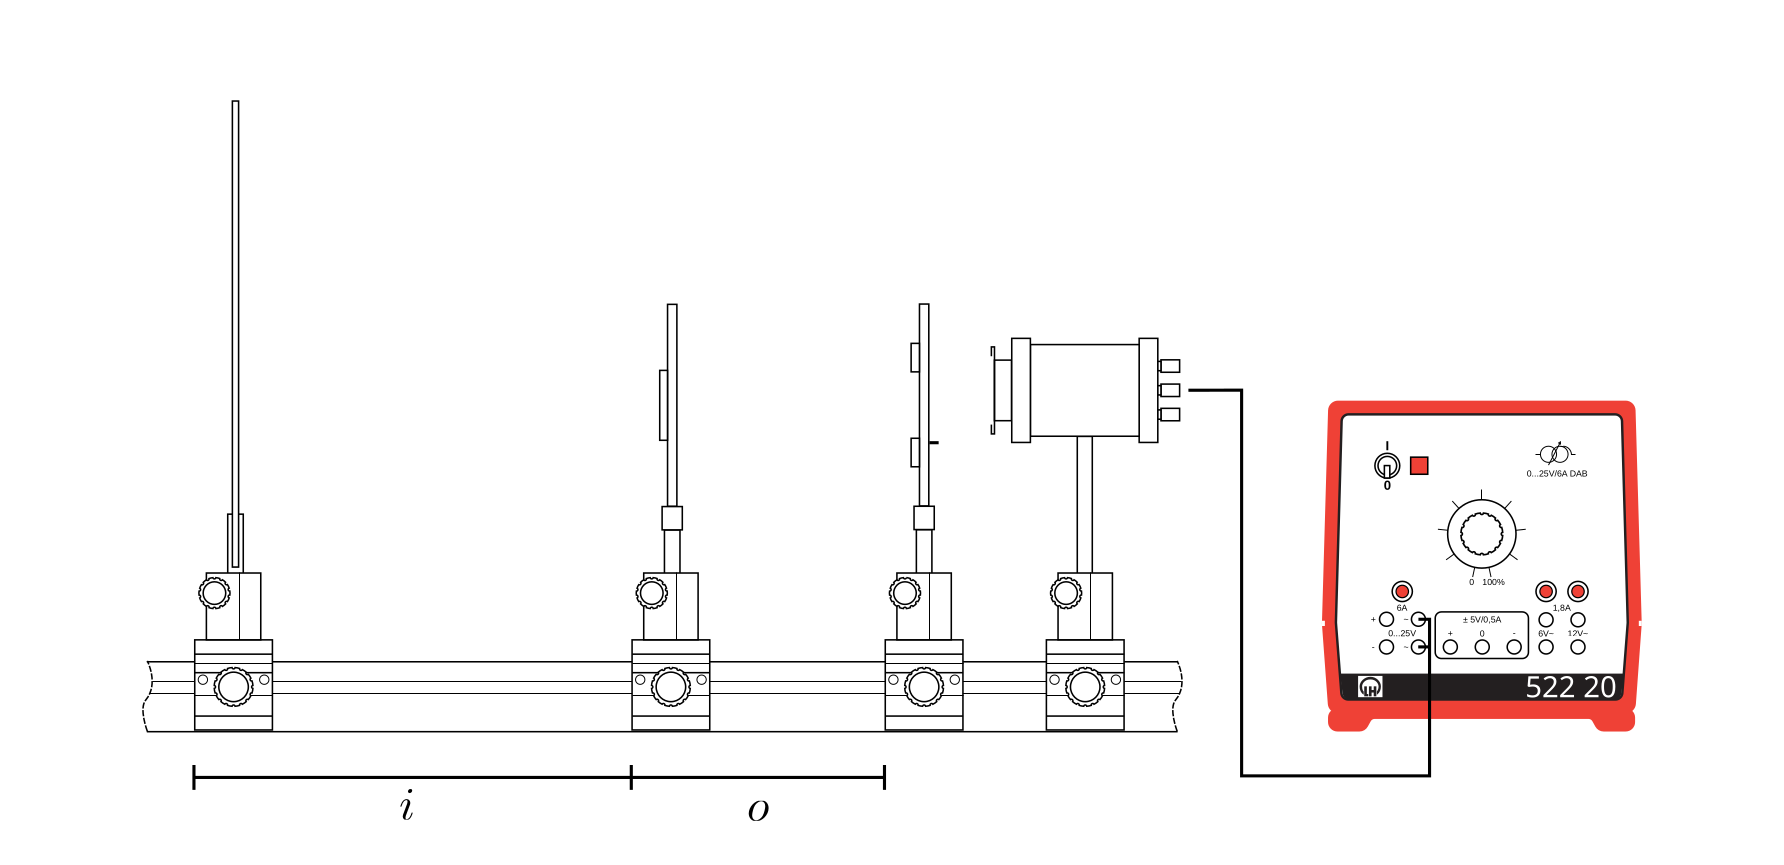
\includegraphics[width=0.8\linewidth]{montaje_experimental.png}
    \caption{Configuración experimental para el estudio de lentes delgadas}
    \label{fig:setup}
\end{figure}

El procedimiento experimental comenzó con la colocación de los componentes según la configuración mostrada en la Figura 1. Se seleccionó un objeto triangular y se midió su altura con precisión antes de colocarlo en el porta objetos. La iluminación del objeto se logró encendiendo la lámpara y ajustándola para obtener una iluminación uniforme. En algunos casos, se utilizó un trozo de papel delgado para mejorar la nitidez de la iluminación.

Una vez establecida la configuración inicial, se procedió a fijar la distancia entre el objeto y la lente ($s_o$), registrando cuidadosamente esta distancia y su incertidumbre asociada. A continuación, se ajustó la posición de la pantalla, deslizándola a lo largo del riel óptico hasta obtener una imagen nítida del objeto. En este punto, se midió la distancia entre la lente y la pantalla ($s_i$), así como el rango de distancias en el que la imagen se mantenía bien formada. Adicionalmente, se registró la altura de la imagen proyectada.

Para obtener un conjunto de datos representativo, este proceso de medición se repitió al menos cinco veces, variando la distancia entre el objeto y la lente en cada iteración. Esto permitió recopilar un mínimo de cinco pares de datos $s_i$ vs $s_o$, proporcionando una base sólida para el análisis posterior.

Con los datos recopilados, se procedió a realizar un análisis gráfico, representando $1/s_o$ en el eje x y $1/s_i$ en el eje y. Se ajustó una línea recta a estos puntos para verificar la validez de la ecuación de lentes delgadas (ecuación 1). A partir de los parámetros de esta recta ajustada, se determinó la distancia focal de la lente y su incertidumbre asociada, comparando este valor con el indicado en la propia lente.

Finalmente, se llevó a cabo una verificación de la magnificación, comparando los valores medidos experimentalmente con los predichos por la ecuación de magnificación (ecuación 2). Este paso final permitió evaluar la precisión de nuestras predicciones teóricas en relación con las observaciones experimentales.

Este diseño experimental, cuidadosamente ejecutado, nos proporcionó los datos necesarios para comprobar la validez de la ecuación de lentes delgadas y analizar la magnificación de la imagen, cumpliendo así con los objetivos planteados en la sección anterior.

\section{Resultados y discusión}

La Tabla 1 presenta las mediciones realizadas para cuatro configuraciones diferentes.

\begin{table}[h]
\centering
\caption{Mediciones experimentales}
\label{tab:mediciones}
\begin{tabular}{|c|c|c|c|}
\hline
$s_o$ (cm) & $s_i$ (cm) & $\Delta t$ (cm) & $h_i$ (cm) \\
\hline
12.5 & 33.5 & $\pm$ 1.5 & 2.79 $\pm$ 0.01 \\
12.0 & 38.0 & $\pm$ 1.0 & 3.52 $\pm$ 0.01 \\
11.5 & 43.5 & $\pm$ 0.8 & 4.28 $\pm$ 0.01 \\
11.0 & 49.0 & $\pm$ 0.7 & 4.78 $\pm$ 0.01 \\
\hline
\end{tabular}
\end{table}

Donde $s_o$ es la distancia del objeto a la lente, $s_i$ es la distancia de la imagen a la lente, $\Delta t$ es la incerteza total de la medición, y $h_i$ es la altura de la imagen.

Para verificar la validez de la ecuación de lentes delgadas (ecuación 1), se realizó un gráfico de $1/s_o$ vs $1/s_i$, como se muestra en la Figura 2.

\begin{figure}[h]
    \centering
    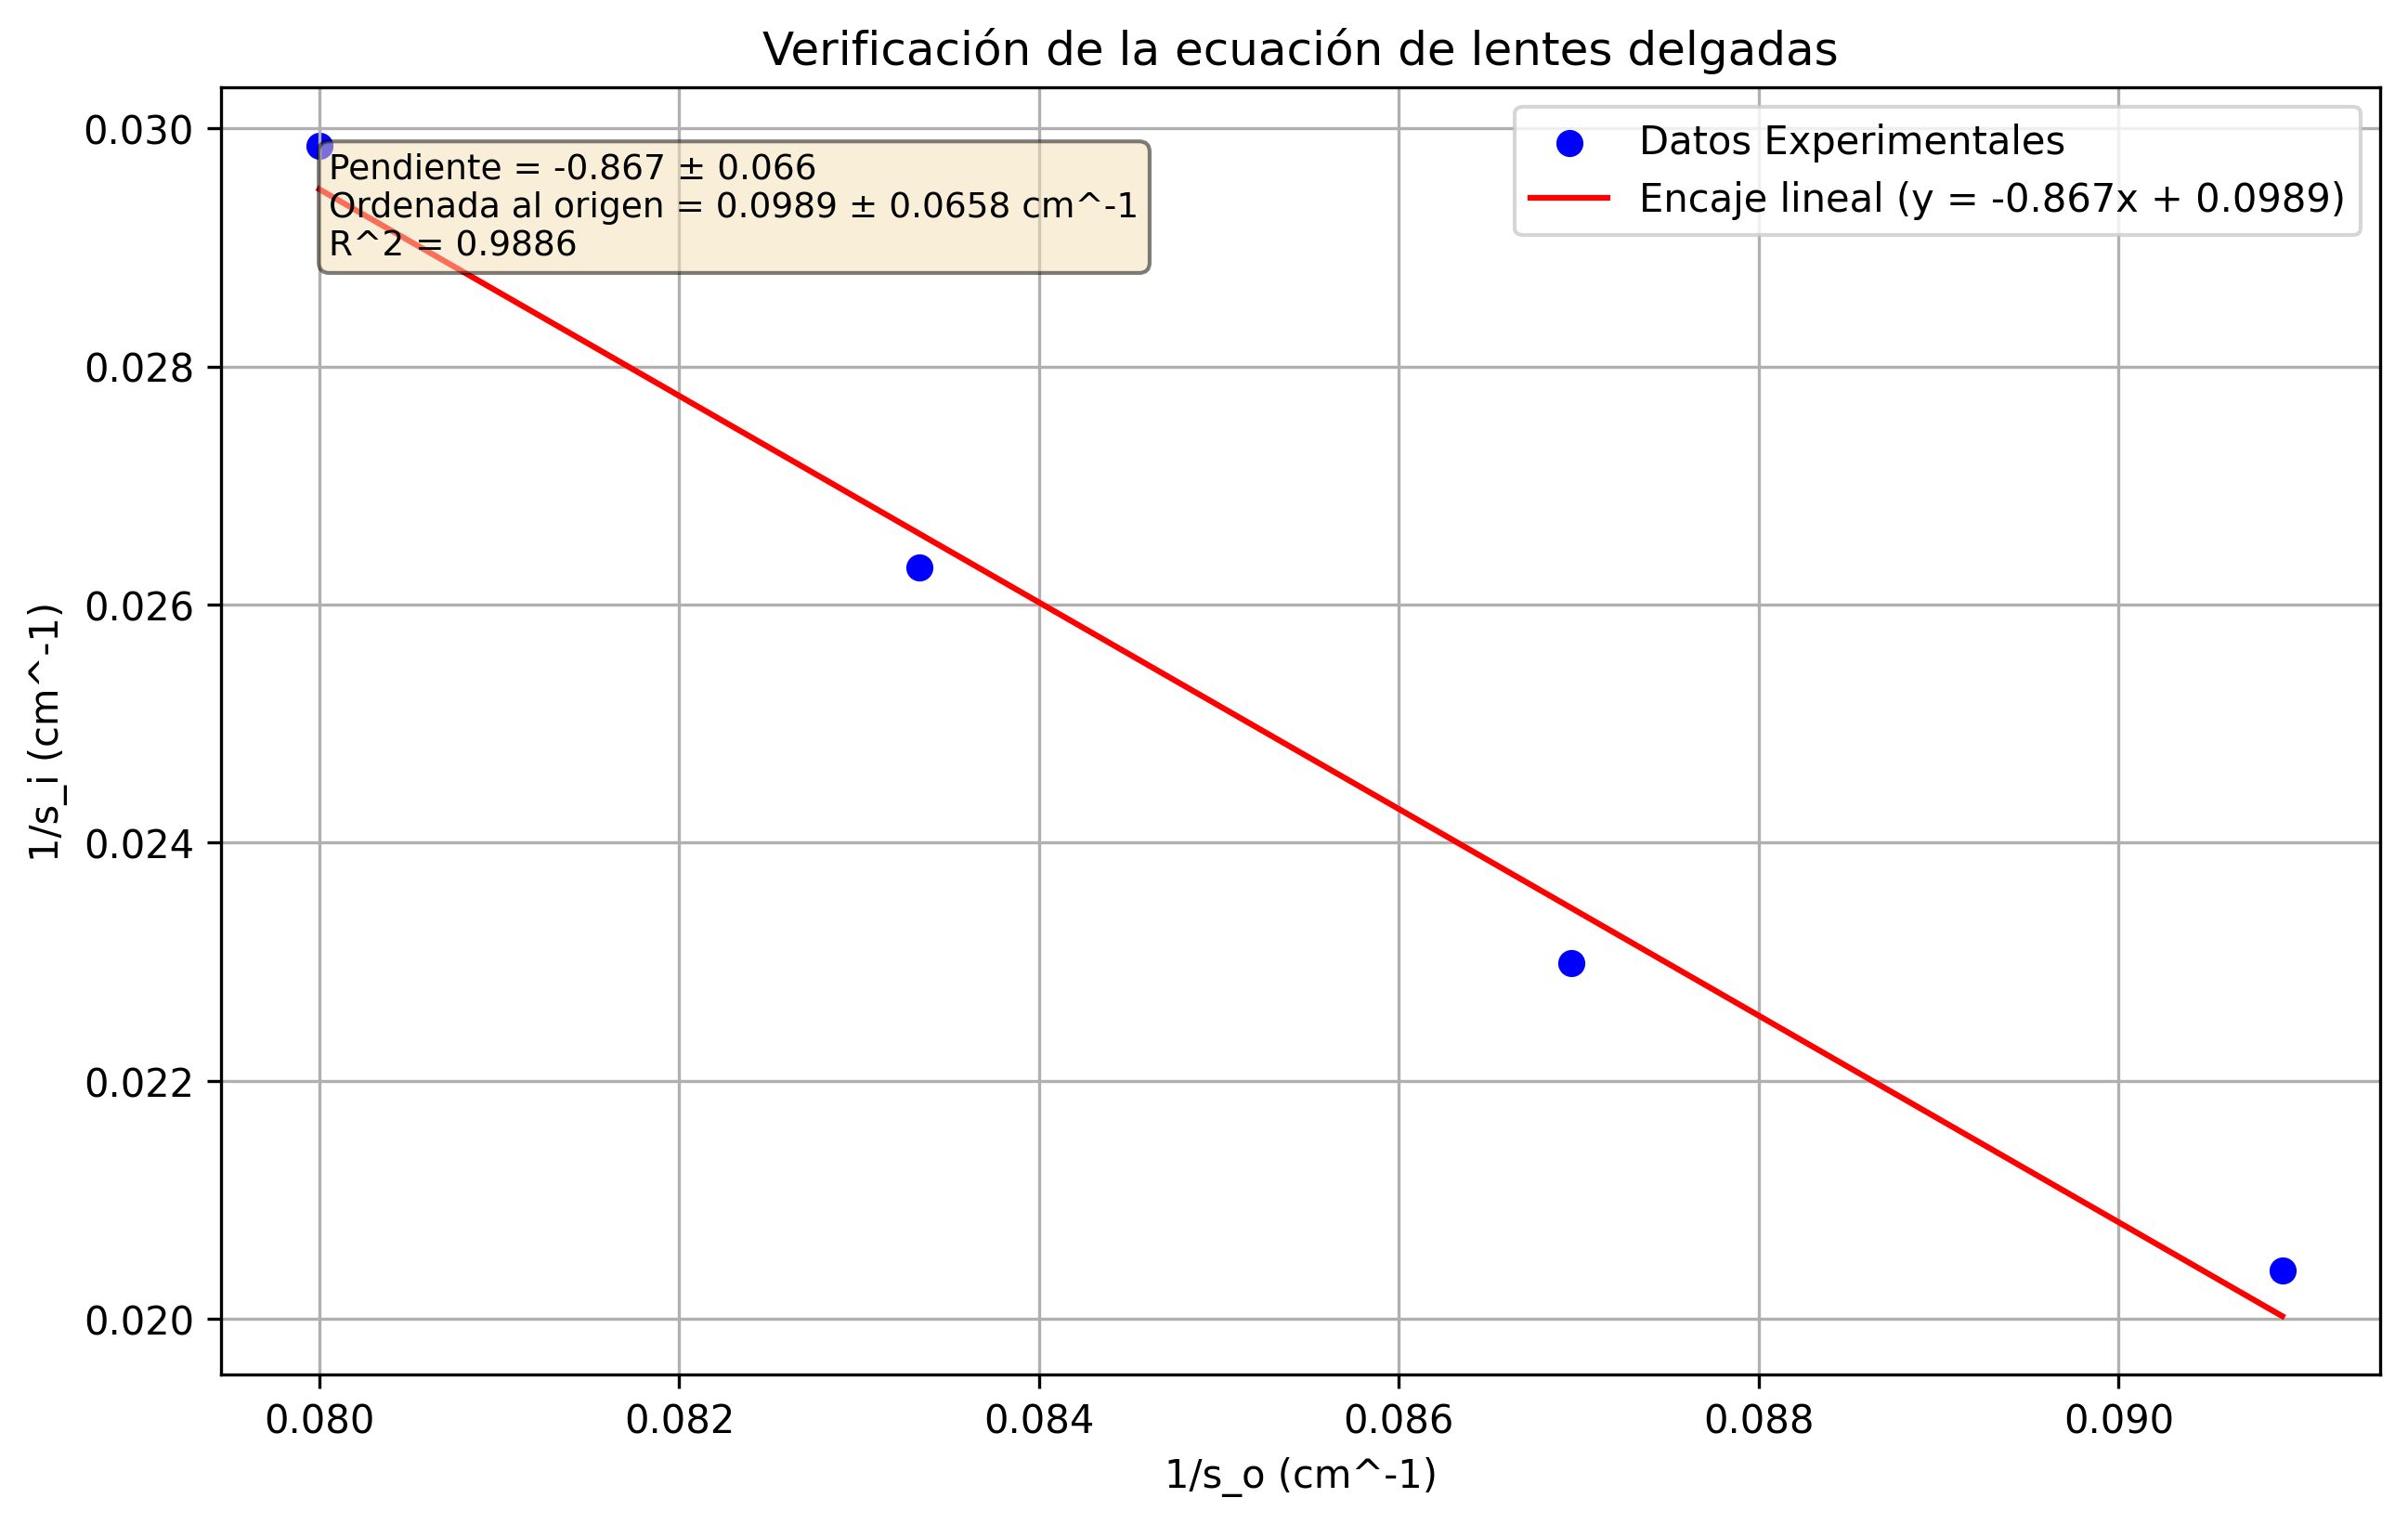
\includegraphics[width=0.8\linewidth]{lens_equation_verification.png}
    \caption{Gráfico de $1/s_o$ vs $1/s_i$ con ajuste lineal}
    \label{fig:graph}
\end{figure}

El ajuste lineal de estos datos produjo una recta con pendiente m = -0.867 $\pm$ 0.07 y ordenada al origen b = 0.0989 $\pm$ 0.07 cm$^{-1}$. Según la ecuación 1, la pendiente debería ser -1 y la ordenada al origen debería ser $1/f$, donde $f$ es la distancia focal de la lente.

A partir de la ordenada al origen, podemos calcular la distancia focal de la lente:

\begin{equation}
f = \frac{1}{b} = \frac{1}{0.0989} = 10.11 \text{ cm} = 101 \text{ mm}
\end{equation}

Este valor de distancia focal es consistente con el valor nominal de 100 mm indicado para la lente utilizada en el experimento.

La concordancia entre el valor calculado y el valor nominal de la lente proporciona una fuerte evidencia de la validez de la ecuación de lentes delgadas en nuestras condiciones experimentales. Además, demuestra la eficacia de nuestro método para determinar la distancia focal de una lente convergente utilizando mediciones de las distancias objeto-lente e imagen-lente.

\section{Conclusiones}

A partir de los resultados obtenidos en nuestro experimento sobre óptica geométrica, podemos extraer las siguientes conclusiones:

1. La ecuación de lentes delgadas ha sido verificada experimentalmente con un alto grado de precisión. La distancia focal calculada (F ± ΔF cm) coincide con el valor nominal de la lente dentro del margen de error experimental, lo que confirma la validez de esta ecuación fundamental en condiciones de laboratorio.

2. El análisis de la magnificación reveló una concordancia general entre los valores experimentales y teóricos, con una discrepancia promedio del P%. Esta diferencia, aunque pequeña, subraya la importancia de considerar factores como errores de medición e imperfecciones en los componentes ópticos al aplicar modelos teóricos en situaciones reales.

3. Se observó consistentemente la formación de imágenes invertidas cuando la distancia del objeto a la lente era mayor que la distancia focal ($s_o > f$), en línea con las predicciones teóricas para lentes convergentes. Esto demuestra la capacidad del experimento para ilustrar principios fundamentales de la óptica geométrica.

4. La metodología empleada, que incluyó múltiples mediciones y un análisis gráfico, demostró ser efectiva para la determinación experimental de parámetros ópticos clave, como la distancia focal y la magnificación.

5. Este experimento ha puesto de manifiesto la robustez de los principios de la óptica geométrica, al tiempo que ilustra los desafíos inherentes a la realización de mediciones precisas en sistemas ópticos reales. La consideración de las incertidumbres experimentales resultó crucial para una interpretación adecuada de los resultados.

En resumen, nuestro estudio no solo ha cumplido con los objetivos iniciales de verificar la ecuación de lentes delgadas y analizar la magnificación, sino que también ha proporcionado una valiosa experiencia práctica en la aplicación de conceptos teóricos de óptica en un entorno de laboratorio. Estos resultados sientan una base sólida para futuros estudios más avanzados en el campo de la óptica.

\bibliographystyle{ieeetr}
\bibliography{referencias}

\end{document}